\documentclass[12pt, a4paper]{article}
\usepackage[utf8]{inputenc}
\usepackage[spanish]{babel}
\usepackage{hyperref}
\usepackage{graphicx}
\usepackage{tabularx}
\usepackage{geometry}
\usepackage{float} % Para asegurar que las imágenes se queden en su lugar con [H]
\geometry{a4paper, margin=2.5cm}

\begin{document}

% --- PORTADA ESTILO UNIVERSIDAD DE CARABOBO ---
\begin{titlepage}
    \centering
    {\large \textbf{UNIVERSIDAD DE CARABOBO}} \\
    {\large \textbf{FACULTAD DE CIENCIAS Y TECNOLOGÍA}} \\
    {\large \textbf{DEPARTAMENTO DE COMPUTACIÓN}} \\
    {\large \textbf{ARQUITECTURA DEL COMPUTADOR}} \\
    
    \vspace{4cm}
    
    {\LARGE \textbf{Simulación del PC de Ciberseguridad}} \\
    
    \vfill
    
    \begin{flushright}
        \begin{tabular}{ll}
            \textbf{Profesor:} & José Canache \\
            \textbf{Integrantes:} & Freddy Ovalle C.I: 31.709.650 \\
                                 & Julián Rebolledo C.I: 29.704.617 \\

        \end{tabular}
    \end{flushright}
    
    \vfill
    
    {\large 26 de mayo de 2026}
\end{titlepage}

\newpage
\pagenumbering{arabic}

% --- CONTENIDO ---
\section*{Argumento}
En la era de la hiperconectividad y la transformación digital masiva, la seguridad de la información ha dejado de ser un complemento de soporte técnico para convertirse en un pilar fundamental de la continuidad operativa y la soberanía tecnológica. A medida que las infraestructuras de red y las arquitecturas de software se vuelven más complejas, las amenazas cibernéticas evolucionan con la misma rapidez, utilizando técnicas de evasión avanzadas que desafían los mecanismos de defensa tradicionales. En este panorama de vulnerabilidad constante, la ciberseguridad ya no puede limitarse a una postura puramente reactiva; exige un enfoque proactivo, estratégico y de bajo nivel.

En este contexto, el hacking ético y el análisis de malware se consolidan como dos disciplinas críticas e interconectadas que permiten entender el ecosistema de las amenazas desde la perspectiva del atacante:

\begin{itemize}
    \item \textbf{Hacking Ético:} Actúa como la primera línea de defensa activa. Al adoptar la mentalidad, metodologías y herramientas de un adversario real, los profesionales de la seguridad logran identificar, explotar y mitigar vulnerabilidades en un entorno controlado antes de que actores maliciosos las aprovechen.
    
    \item \textbf{Análisis de Malware:} Representa la ingeniería forense del conflicto digital. Cuando un código malicioso logra vulnerar el perímetro, el análisis técnico -tanto estático como dinámico- permite desglosar el comportamiento del ejecutable, comprender su interacción con el sistema operativo, identificar sus mecanismos de persistencia y desentrañar sus vectores de comunicación.
\end{itemize}

Mientras el hacking ético define cómo entran los atacantes a un sistema, el análisis de malware revela exactamente qué hacen una vez que están adentro y cómo operan a nivel de instrucciones y memoria.

\newpage
\section*{Componentes del Sistema}

\subsection*{CPU}
El AMD Ryzen 9 9950X es el cerebro absoluto de la operación. Con 16 núcleos físicos y 32 hilos de procesamiento basados en la arquitectura Zen 5, este procesador de gama entusiasta no solo procesa datos; está diseñado para triturar cargas de trabajo paralelas masivas, lo que lo convierte en la herramienta definitiva para simular infraestructuras empresariales enteras y diseccionar las amenazas digitales más complejas.

\begin{itemize}
    \item \textbf{La Cúspide de la Virtualización Masiva (Multi-Tasking Extremo):} Con 32 hilos de procesamiento, se puede diseñar un entorno de red hiperrealista en un hipervisor. Se puede asignar, por ejemplo: 8 hilos para un controlador de dominio Windows Server (Active Directory). 4 hilos para una máquina de análisis estático (Flare-VM). 4 hilos para una máquina de análisis dinámico de red (REMnux). 4 hilos para tu máquina atacante (Kali Linux). Y aún te quedarán 12 hilos libres en el sistema anfitrión (host) para compilar código, navegar o registrar logs sin pestañear.
    \item \textbf{Fuzzing de Código a Alta Velocidad:} El fuzzing de binarios (probar miles de combinaciones de entrada por segundo para colapsar un programa y hallar vulnerabilidades) se beneficia directamente del brutal rendimiento multihilo y de las instrucciones AVX-512 nativas de este chip. Con herramientas como AFL++, reducirás el tiempo de descubrimiento de exploits de días a solo horas.
\end{itemize}

\begin{figure}[H]
    \centering
    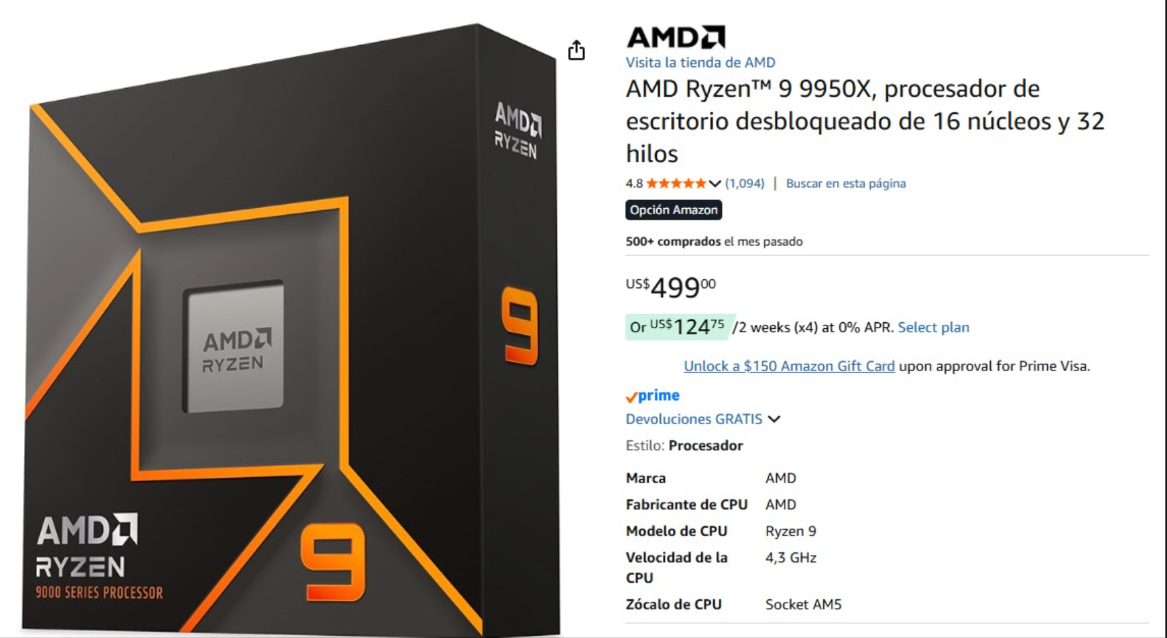
\includegraphics[width=0.5\textwidth]{cpu.png}
\end{figure}
\newpage

\subsection*{Memoria RAM}
Para un hacker ético o un analista de malware, la memoria RAM no es un lujo estético; es el músculo que sostiene los entornos aislados, las herramientas de ingeniería inversa y los laboratorios virtuales complejos. El kit G.SKILL Trident Z5 RGB DDR5 de 64GB (2x32GB) a 6000MT/s ofrece la capacidad masiva y la velocidad extrema necesarias para ejecutar operaciones de seguridad ofensiva y defensiva sin cuellos de botella.

\begin{itemize}
    \item \textbf{64GB de Capacidad (El Paraíso de la Virtualización):} El análisis de malware moderno exige el uso de entornos cerrados (sandboxes). Con 64GB de memoria, puedes levantar simultáneamente un dominio completo de Active Directory para simular ataques de pentesting, una máquina atacante con Kali Linux, y múltiples entornos de análisis aislados (Flare-VM o REMnux) sin que el sistema operativo anfitrión sufra la más mínima ralentización.
    \item \textbf{Velocidad de 6000 MT/s y Latencia CL30 (Respuesta Inmediata):} La baja latencia estructural (CL30) y la velocidad de la tecnología DDR5 aceleran exponencialmente los procesos de computación intensiva. Esto se traduce en un procesamiento y descompilación de binarios mucho más rápido en herramientas como IDA Pro, Ghidra o Radare2, permitiendo saltar entre funciones de código malicioso de forma instantánea.
    \item \textbf{Análisis Forense de Memoria Volátil (RAM Forensics):} Al trabajar con herramientas como Volatility para analizar volcados de memoria de sistemas comprometidos por rootkits o ransomware, la velocidad de transferencia de datos de este kit agiliza la búsqueda de procesos ocultos, sockets abiertos e inyecciones de código en segundos.
\end{itemize}

\begin{figure}[H]
    \centering
    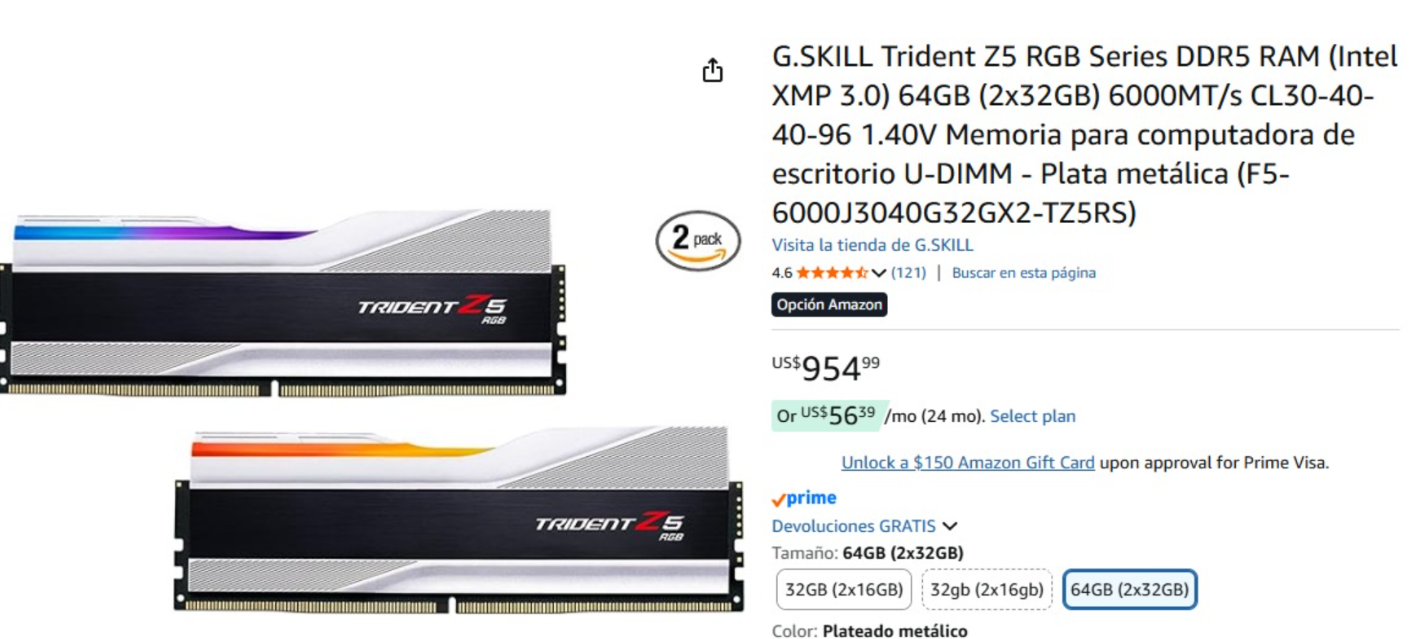
\includegraphics[width=0.5\textwidth]{ra,.png}
\end{figure}
\newpage

\subsection*{Placa Base}
La MSI MAG X670E Tomahawk WiFi (Plataforma AMD AM5) no es solo una placa para jugar; es una estación de control de nivel de servidor doméstico, diseñada para orquestar de manera segura el tráfico de datos, la virtualización y el hardware de alta gama.

\begin{itemize}
    \item \textbf{Arquitectura AM5 y Chipset X670E (Virtualización sin Límites):} Para levantar hipervisores complejos (Proxmox, VMware Workstation o Hyper-V), necesitas una placa con excelente soporte para AMD-V e IOMMU. El chipset X670E permite la segmentación avanzada de hardware, lo que significa que puedes hacer passthrough (pasar el control directo) de tarjetas de red físicas o GPUs directamente a tus máquinas virtuales de análisis de malware o Kali Linux, aislándolas por completo del sistema operativo anfitrión.
    \item \textbf{Velocidad de Respuesta Excepcional para Snapshots de Máquinas Virtuales:} Cuando detonas un ransomware o un troyano en tu Sandbox, el sistema operativo virtualizado queda destruido o comprometido. Gracias a sus múltiples ranuras M.2 PCIe (incluyendo soporte PCIe 5.0), puedes instalar unidades NVMe ultrarrápidas para revertir las máquinas virtuales a su estado limpio (snapshot) en cuestión de un par de segundos.
    \item \textbf{Segmentación Física de Redes:} Cuenta con un puerto LAN de 2.5 Gbps y conectividad Wi-Fi 6E lo Permite realizar auditorías de redes inalámbricas y capturas de tráfico masivo (análisis de paquetes con Wireshark) sin pérdida de frames.
\end{itemize}

\begin{figure}[H]
    \centering
    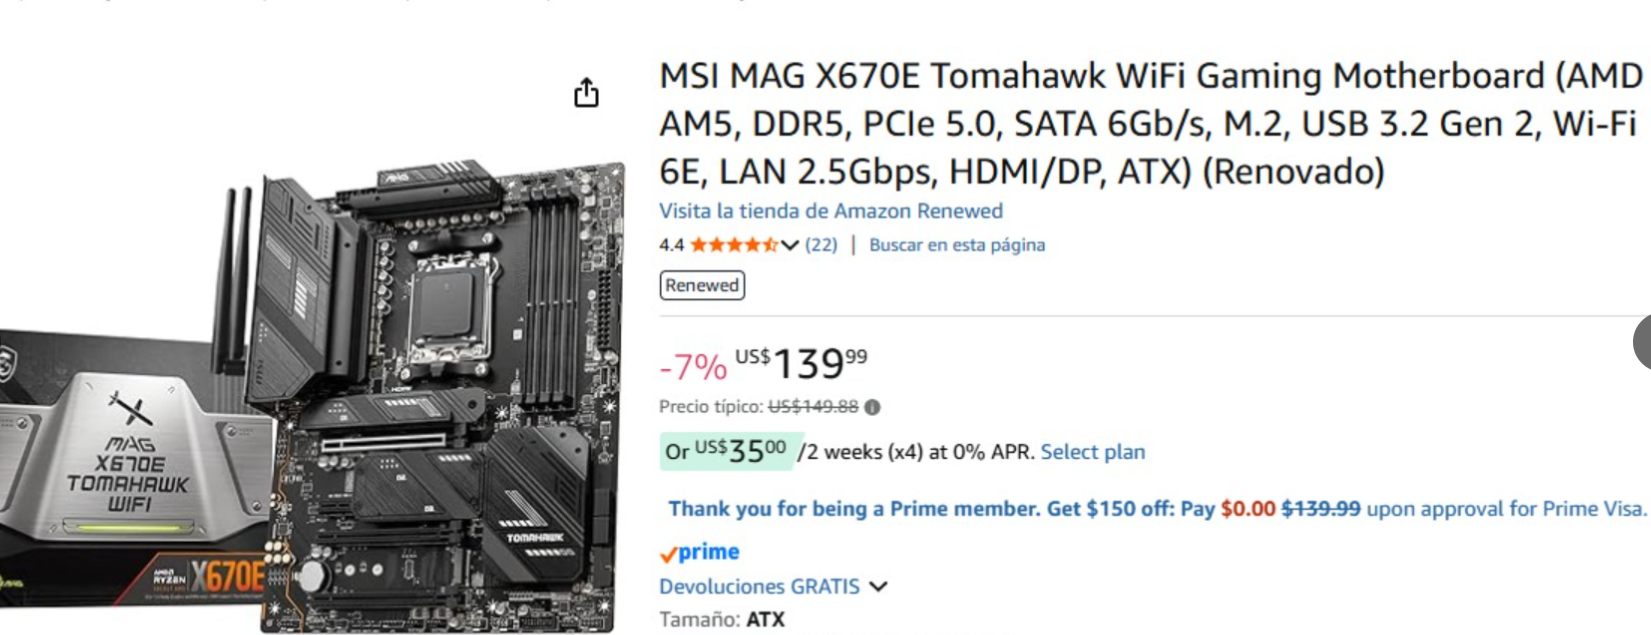
\includegraphics[width=0.5\textwidth]{placa.png}
\end{figure}
\newpage

\subsection*{Almacenamiento Principal}
Como almacenamiento principal, el Acer Predator GM7000 M.2 NVMe de 2TB no solo guarda los archivos; es el responsable de dictar la velocidad con la que arranca el sistema operativo anfitrión (host), la fluidez de las herramientas forenses y la velocidad de respuesta de los discos virtuales. Con velocidades de lectura de 7400 MB/s gracias a la interfaz PCIe Gen4x4, este componente elimina el cuello de botella más común en la virtualización pesada: el tiempo de espera de disco.

\begin{figure}[H]
    \centering
    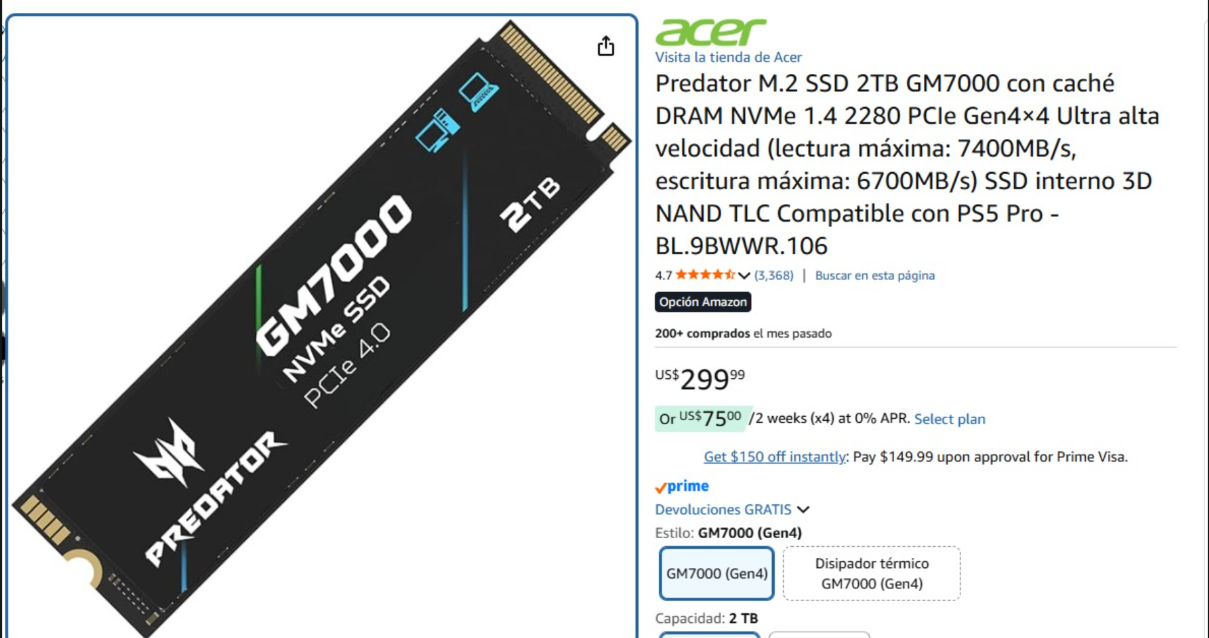
\includegraphics[width=0.5\textwidth]{ssdprincipal.png}
\end{figure}

\subsection*{Almacenamiento Secundario}
El almacenamiento secundario cumple una función de contención y organización crítica. El Kingston NV3 de 1TB M.2 NVMe PCIe 4.0 ofrece una velocidad de hasta 6000 MB/s, consolidándose como la unidad ideal para actuar como "búnker" de archivos pesados, librerías de sistemas operativos y bases de datos analíticas, aliviando la carga del disco principal.

\begin{figure}[H]
    \centering
    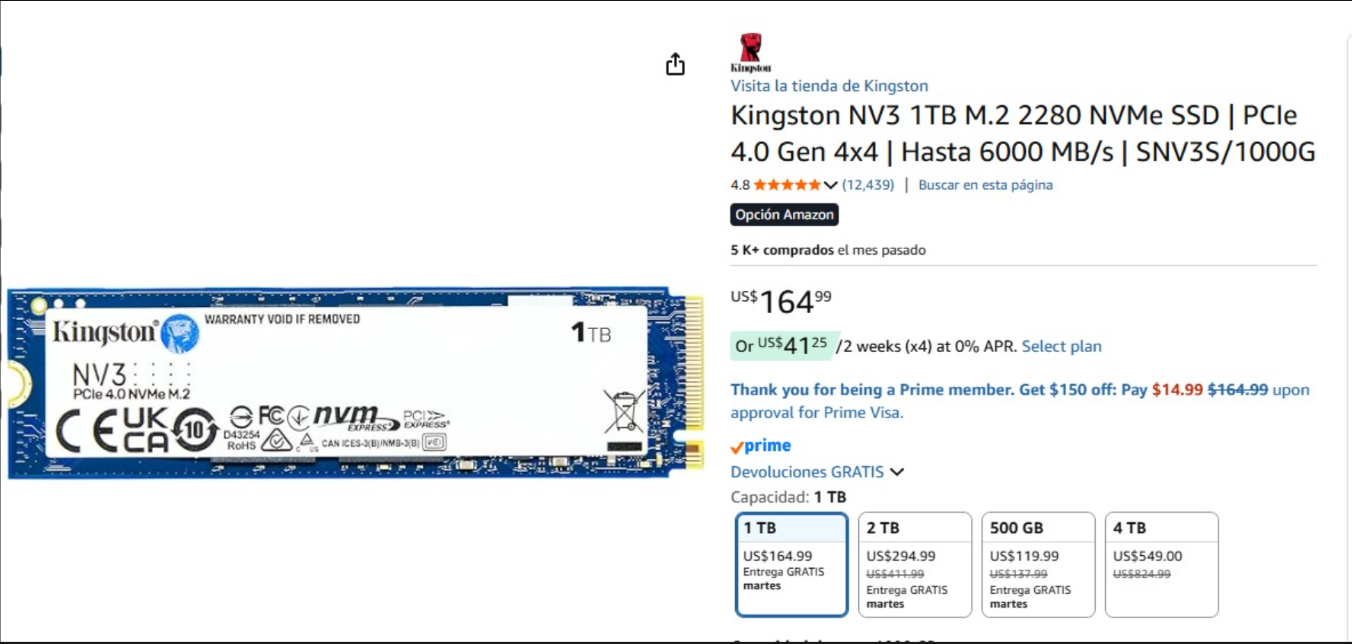
\includegraphics[width=0.5\textwidth]{ssdrespaldo.png}
\end{figure}
\newpage

\subsection*{GPU}
La MSI Gaming RTX 5070 de 12GB, impulsada por la arquitectura de vanguardia NVIDIA Blackwell, es la pieza encargada de ejecutar auditorías de contraseñas por fuerza bruta y procesar modelos locales de Inteligencia Artificial aplicados a la detección de anomalías en tiempo récord.

\begin{itemize}
    \item \textbf{Rompiendo Cifrados a Velocidades de Vértigo (Hash Cracking):} El uso principal de una GPU en seguridad ofensiva es la auditoría de credenciales. Al ejecutar herramientas como Hashcat o John the Ripper, los miles de núcleos CUDA de la arquitectura Blackwell procesan algoritmos matemáticos en paralelo. Esto permite probar miles de millones de combinaciones por segundo al intentar descifrar hashes de contraseñas, reduciendo ataques que a una CPU le tomarían años a solo unas pocas horas.
    \item \textbf{Arquitectura Blackwell y Tensor Cores (Ciberseguridad Asistida por IA):} La inclusión de núcleos Tensor de última generación permite desplegar en un laboratorio modelos de lenguaje locales (LLMs compactos) o redes neuronales entrenadas para la seguridad.
    \item \textbf{Memoria GDDR7 (El Salto en Ancho de Banda):} Esta tarjeta introduce la tecnología GDDR7, que ofrece una velocidad de transferencia y un ancho de banda masivamente superior a las generaciones anteriores.
\end{itemize}

\begin{figure}[H]
    \centering
    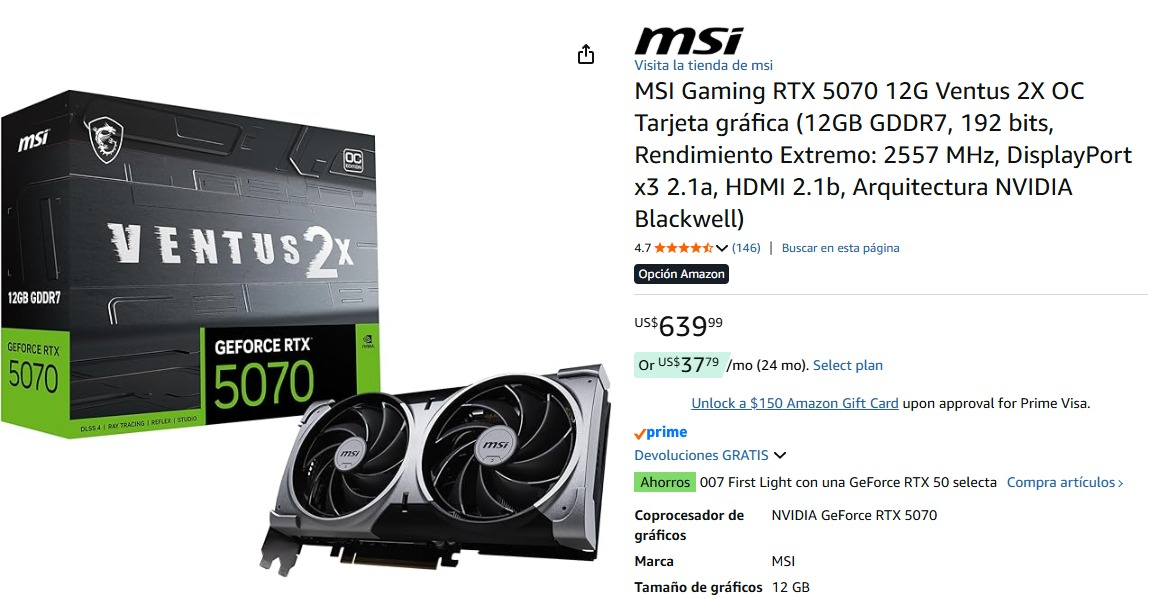
\includegraphics[width=0.5\textwidth]{WhatsApp Image 2026-05-22 at 22.08.25.jpeg}
\end{figure}
\newpage

\subsection*{Fuente de Poder}
La fuente Auotac de 1000W Totalmente Modular proporciona el flujo eléctrico masivo, limpio y protegido que exige un laboratorio diseñado para operar bajo estrés continuo durante horas o días.

\begin{itemize}
    \item Tener una fuente de 1000W significa que operarás exactamente en el punto dulce de eficiencia, garantizando que los componentes internos de la fuente sufran el menor desgaste posible con el paso de los años. Esta fuente tiene Potencia de sobra para alimentar el Ryzen 9 9950X y la RTX 5070 a máxima carga simultánea.
\end{itemize}

\begin{figure}[H]
    \centering
    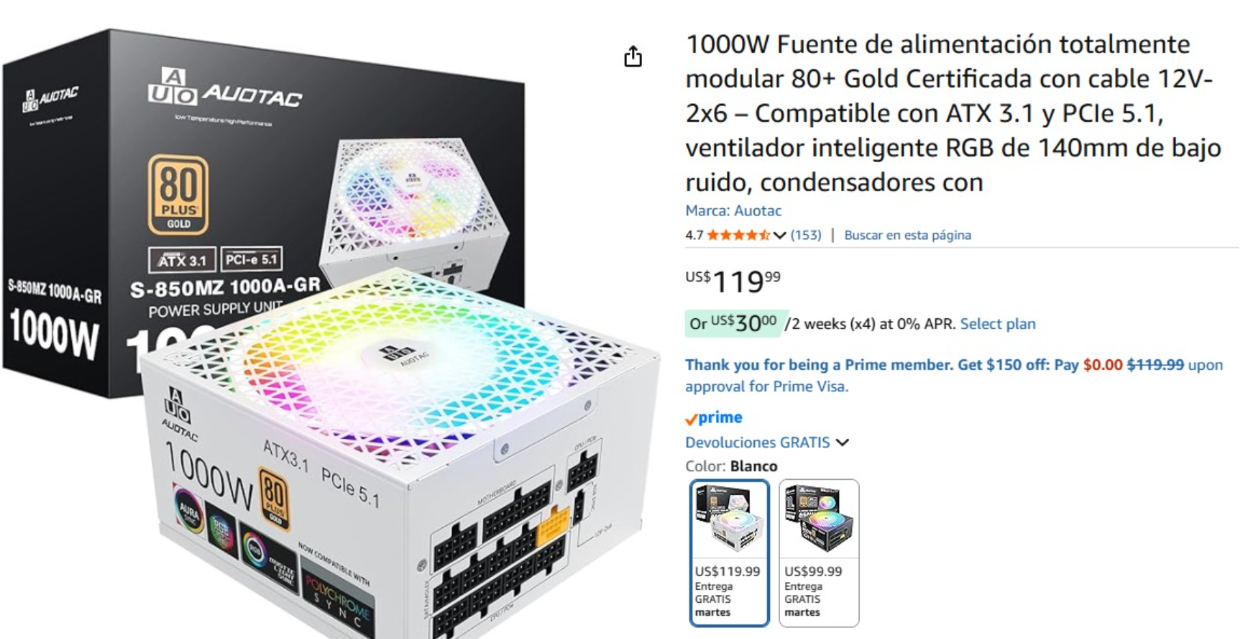
\includegraphics[width=0.5\textwidth]{fuente.png}
\end{figure}

\subsection*{Refrigeración}
El ARCTIC Liquid Freezer III Pro 360 no es un simple accesorio estético; es el escudo térmico indispensable para garantizar la estabilidad del sistema operativo anfitrión (host) cuando se somete a la CPU a cargas de trabajo críticas, prolongadas y de estrés extremo. Al momento de que el procesador trabaje al 100\%, el radiador es capaz de disipar el calor de manera eficiente, evitando bajada de potencia por sobrecalentamiento y manteniendo el rendimiento de ataque al máximo.

\begin{figure}[H]
    \centering
    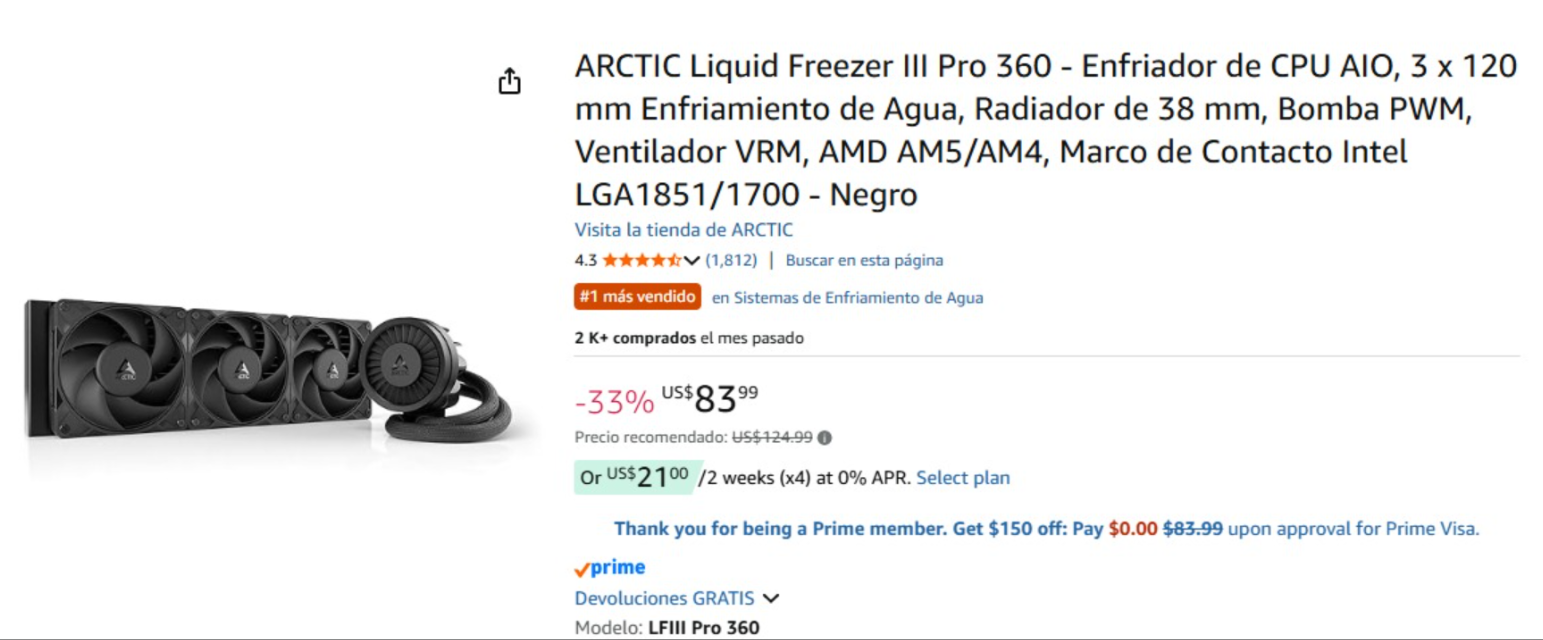
\includegraphics[width=0.5\textwidth]{liquida.png}
\end{figure}
\newpage

\subsection*{Case}
El gabinete es el chasis que unifica la infraestructura, garantizando el flujo de aire y añadiendo una capa de monitoreo físico directo. El RAIDMAX 1803 no es solo una torre con estética moderna; es una cabina de control espaciosa diseñada para albergar componentes de gran escala bajo estrictas demandas de ventilación. Este gabinete cuenta con una pantalla LCD que permite ver las métricas tanto como el procesador, memoria ram, etc.

\begin{figure}[H]
    \centering
    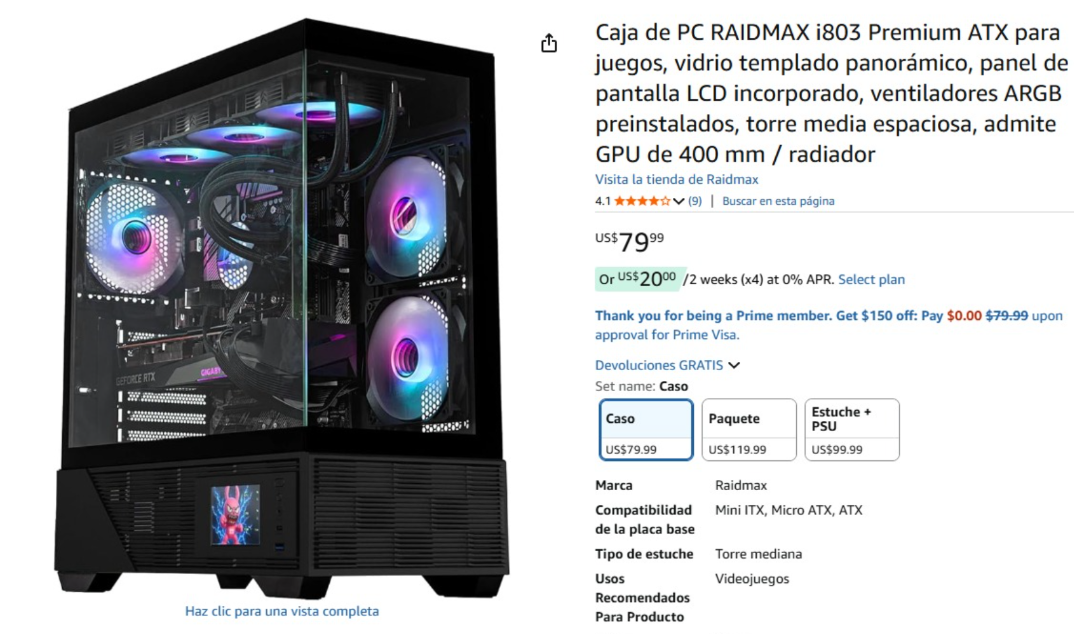
\includegraphics[width=0.5\textwidth]{case.png}
\end{figure}

\subsection*{Pasta Térmica}
La Noctua NT-H1 de 10 gramos es un compuesto térmico de grado profesional aclamado por su durabilidad y baja resistencia térmica, actuando como el puente conductor crítico entre el procesador y el bloque de enfriamiento por agua.

\begin{figure}[H]
    \centering
    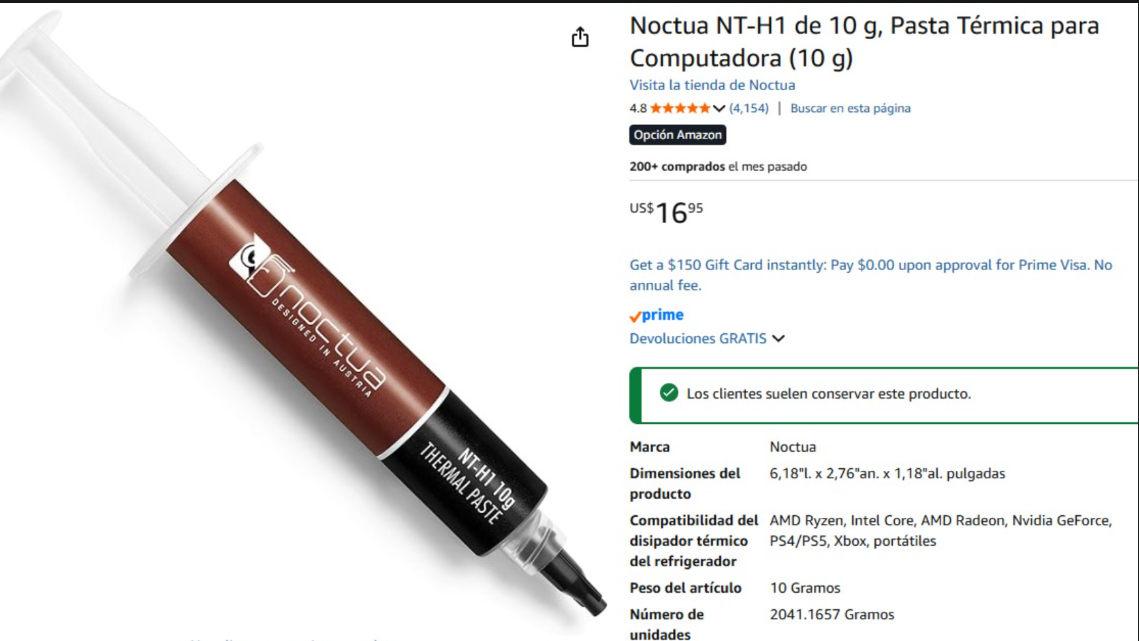
\includegraphics[width=0.5\textwidth]{pasta.png}
\end{figure}

\newpage
\section*{Presupuesto y Enlaces}

\begin{table}[htbp]
\centering
\resizebox{\textwidth}{!}{
\begin{tabular}{|l|l|l|}
\hline
\textbf{Componente} & \textbf{Modelo} & \textbf{Precio} \\ \hline
CPU & AMD Ryzen™ 9 9950X & \$499.00 \\ \hline
Memoria RAM & G.SKILL Trident Z5 RGB Series DDR5 RAM 64GB (2x32GB) & \$954.99 \\ \hline
GPU & MSI Gaming RTX 5070 12G Ventus 2X OC & \$639.99 \\ \hline
Placa Base & MSI MAG X670E Tomahawk WiFi Gaming & \$139.99 \\ \hline
Almacenamiento (Principal) & Predator M.2 SSD 2TB GM7000 DRAM NVMe & \$299.99 \\ \hline
Almacenamiento (Secundario) & Kingston NV3 1TB M.2 2280 NVMe SSD & \$164.99 \\ \hline
Case & RAIDMAX 1803 Premium ATX & \$79.99 \\ \hline
Fuente de Poder & AUOTAC S-850MZ 1000A-GR & \$119.99 \\ \hline
Refrigeración & ARCTIC Liquid Freezer III Pro 360 & \$83.99 \\ \hline
Pasta Térmica & Noctua NT-H1 de 10 g & \$16.95 \\ \hline
\textbf{Total} & & \textbf{\$2,999.87} \\ \hline
\end{tabular}
}
\end{table}

\subsection*{Enlaces}
\begin{itemize}
    \item \textbf{Almacenamiento (Principal):} \url{https://www.amazon.com/-/es/gp/product/B09F5W62N8/ref=ox_sc_act_image_10?smid=A37TNC2POOX0TX&th=1}
    \item \textbf{CPU:} \url{https://www.amazon.com/-/es/gp/product/B0D6NNRBGP/ref=ox_sc_act_image_9?smid=ATVPDKIKX0DER&th=1}
    \item \textbf{Placa base:} \url{https://www.amazon.com/-/es/gp/product/B0CLMJ2RCR/ref=ox_sc_act_image_8?smid=A1CG7B1P8V4L63&th=1}
    \item \textbf{Refrigeración:} \url{https://www.amazon.com/-/es/gp/product/B0DLWGG85P/ref=ox_sc_act_image_7?smid=A2T6N244WTLWGU&th=1}
    \item \textbf{RAM:} \url{https://www.amazon.com/-/es/gp/product/B0B2V9W5KQ/ref=ox_sc_act_image_6?smid=A3TOECTKC4OEBD&th=1}
    \item \textbf{GPU:} \url{https://www.amazon.com/-/es/gp/product/B0DYGDT9YD/ref=ox_sc_act_image_5?smid=ATVPDKIKX0DER&psc=1}
    \item \textbf{Almacenamiento (Secundario):} \url{https://www.amazon.com/-/es/gp/product/B0DBR3DZWG/ref=ox_sc_act_image_4?smid=ATVPDKIKX0DER&th=1}
    \item \textbf{Fuente de Poder:} \url{https://www.amazon.com/-/es/gp/product/B0FDVKG369/ref=ox_sc_act_image_3?smid=A14TD26AEVZUM2&th=1}
    \item \textbf{Case:} \url{https://www.amazon.com/-/es/gp/product/B0FW4RRVTX/ref=ox_sc_act_image_2?smid=A3C6CB26X6LCVO&th=1}
    \item \textbf{Pasta Térmica:} \url{https://www.amazon.com/-/es/gp/product/B07MZ4JJWX/ref=ox_sc_act_image_1?smid=A1Z5H6ZGWCMTNX&psc=1}
\end{itemize}

\newpage
\section*{Conclusión}
Este proyecto de hardware demuestra con éxito cómo un presupuesto inteligente por debajo de los \$3000 es más que suficiente para edificar una estación de trabajo de categoría profesional (Workstation) optimizada para el hacking ético y la ciberseguridad ofensiva y defensiva. En este ámbito, disciplinas críticas como la ingeniería inversa, el fuzzing de binarios y el análisis heurístico de amenazas exigen un ecosistema informático con una potencia de procesamiento paralelo masiva, disponibilidad ininterrumpida y capacidad de diagnóstico en tiempo real.

Dada la alta demanda de procesamiento de datos, análisis en tiempo real y la necesidad de manejar múltiples máquinas virtuales y contenedores, los componentes seleccionados debían garantizar un rendimiento superior y una estabilidad duradera. Una computadora prefabricada simplemente no podría ofrecer la optimización necesaria para estas tareas tan específicas. Por lo tanto, armar un equipo personalizado fue la mejor opción para cumplir con los altos estándares profesionales de esta disciplina. Este enfoque asegura un ambiente de trabajo confiable, escalable y seguro, esencial para estudiar y aplicar habilidades de hacking ético, fortaleciendo así la protección de sistemas reales contra las amenazas emergentes.

Este laboratorio personalizado no solo representa una inversión financiera optimizada y eficiente, sino que establece un entorno de simulación altamente seguro, confiable y escalable. Es la herramienta de ingeniería definitiva para estudiar vulnerabilidades, diseñar contramedidas efectivas y anticiparse con éxito a las amenazas digitales emergentes en el mundo real.

\end{document}